\documentclass[lettersize,journal]{IEEEtran}
\usepackage{bm}
\usepackage{calc}
\usepackage{algorithm2e}
\usepackage{array}
\usepackage{booktabs}
\usepackage{colortbl}
\usepackage{supertabular}
\usepackage{amsmath,amsfonts}
\usepackage{tikz}
\usepackage{subfig}
\hyphenation{op-tical net-works semi-conduc-tor IEEE-Xplore}
\def\BibTeX{{\rm B\kern-.05em{\sc i\kern-.025em b}\kern-.08em
    T\kern-.1667em\lower.7ex\hbox{E}\kern-.125emX}}
\usepackage{balance}
\usepackage[backend=bibtex, style=numeric, sorting=none]{biblatex}
\bibliography{references}

\begin{document}
\title{A Light Weight Approach to Minimize Charging Cost for Electric Bus Fleets}
\author{Daniel Mortensen, Jacob Gunther\thanks{}}

\markboth{Transactions on Intelligent Transportation Systems}%
{}

\maketitle 
\begin{abstract}
\textcolor{red}{Insert abstract here}
\end{abstract}

\begin{IEEEkeywords}
\textcolor{red}{Insert keywords here}
\end{IEEEkeywords}

\section{Introduction}
\textcolor{red}{Insert Introduction Here}

% imports 
\begin{table*}
\centering
\caption{Description of the billing structure}
\begin{tabular}{c | c c c}
		                   & On-Peak                & Off-Peak               & Facilities (Both)\\ \hline
		Energy Rate        & \$ 0.058282  /kWh & \$ 0.029624 /kWh  & None \\
		Energy Rate Symbol & $\mu_{\text{e-on}}$    & $\mu_{\text{e-off}}$   & None \\ \hline
		Power Rate  & \$ 15.73 /kW           & None                   & \$ 4.81 /kW \\
		Power Rate Symbol  & $\mu_{\text{p-on}}$    & None            & $\mu_{\text{p-all}}$
	\end{tabular}
	\label{tab:charges} 
\end{table*}

 
\begin{figure*}
\centering
\scalebox{0.8}{
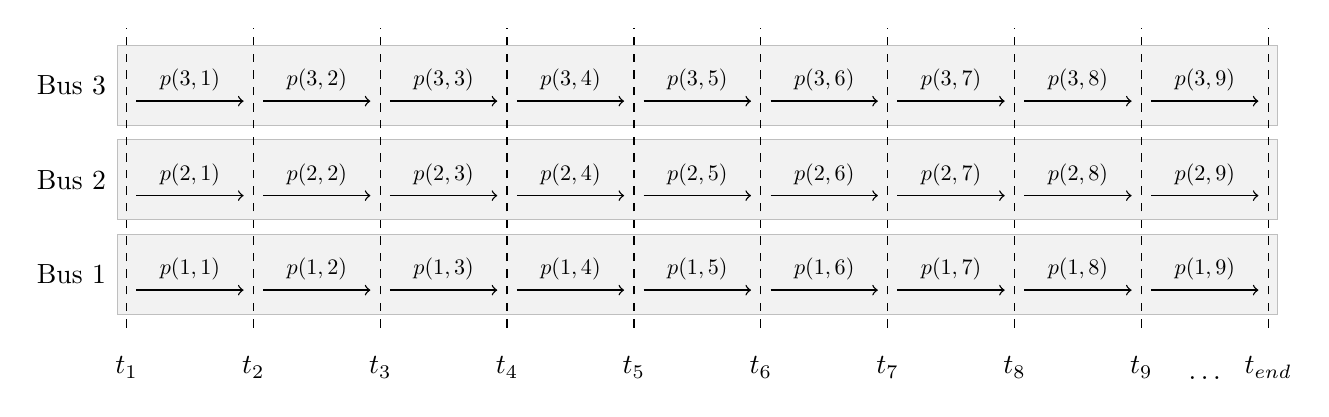
\begin{tikzpicture}
	\node[rectangle, draw=gray!50, fill=gray!10, minimum width=5.8in, minimum height=0.4in](bus1Box) at (7.75,0.8){};
	\node(bus1BoxLabel) at (-0.2, 0.8){Bus 1}; 
	
	\node[rectangle, draw=gray!50, fill=gray!10, minimum width=5.8in, minimum height=0.4in](bus2Box) at (7.75,2){};
	\node(bus1BoxLabel) at (-0.2, 2.0){Bus 2};
	
	\node[rectangle, draw=gray!50, fill=gray!10, minimum width=5.8in, minimum height=0.4in](bus3Box) at (7.75,3.2){};
	\node(bus1BoxLabel) at (-0.2, 3.2){Bus 3};
	
	\foreach \curLab/\preLab[count=\c, evaluate=\c as \pos using {0.5 + (\c - 1)*14.5/9}] in {t_1/t_1, t_2/t_1, t_3/t_2, t_4/t_3, t_5/t_4, t_6/t_7, t_7/t_6, t_8/t_7, t_9/t_8, t_{end}/t_9}
	{
		\node[label=below:$\curLab$](b\c) at (\pos, 0){};
		\node(t) at (\pos, 3.8){};
		\draw[dashed, line width=0.5pt] (b\c.north) -- (t.north); 
		\ifnum\c>1 
			\node(b1Curr) at (\pos, 0.8 - 0.2){};
			\node(b2Curr) at (\pos, 2.0 - 0.2){};
			\node(b3Curr) at (\pos, 3.2 - 0.2){};
			\def\temp{\number\numexpr\c - 1}
			\draw[->, line width=0.5pt] (b1Prev.east) -- node[midway, above]{\scalebox{0.8}{$p(1,\temp)$}}(b1Curr.west);
			\draw[->, line width=0.5pt] (b2Prev.east) -- node[midway, above]{\scalebox{0.8}{$p(2,\temp)$}}(b2Curr.west);
			\draw[->, line width=0.5pt] (b3Prev.east) -- node[midway, above]{\scalebox{0.8}{$p(3,\temp)$}}(b3Curr.west);	
		\fi
			\node(b1Prev) at (\pos, 0.8 - 0.2){};
			\node(b2Prev) at (\pos, 2.0 - 0.2){};
			\node(b3Prev) at (\pos, 3.2 - 0.2){};	
	}
	\path (b9.south) -- node[midway, below=0.1in]{$\hdots$}(b10.south);

\end{tikzpicture}}
\caption{Demonstrates how bus power use is conceptualized}
\label{fig:busPower}
\end{figure*}


\begin{figure*}
\centering
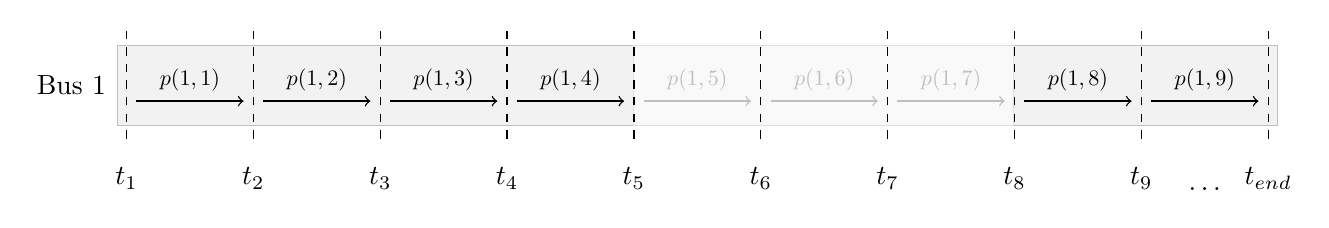
\begin{tikzpicture}
	\node[rectangle, draw=gray!50, fill=gray!10, minimum width=5.8in, minimum height=0.4in](bus1Box) at (7.75,0.8){};
	\node(bus1BoxLabel) at (-0.2, 0.8){Bus 1}; 
	\node[rectangle, draw=gray!25, fill=gray!5, minimum width=1.9in, minimum height=0.4in](bus1Box) at (7.75 + 1.6,0.8){};
	
	\foreach \curLab/\preLab[count=\c, evaluate=\c as \pos using {0.5 + (\c - 1)*14.5/9}] in {t_1/t_1, t_2/t_1, t_3/t_2, t_4/t_3, t_5/t_4, t_6/t_5, t_7/t_6, t_8/t_7, t_9/t_8, t_{end}/t_9}
	{
		\node[label=below:$\curLab$](b\c) at (\pos, 0){};
		\node(t) at (\pos, 1.4){};
		\ifnum\c>1 
			\node(b1Curr) at (\pos, 0.8 - 0.2){};
				\ifnum\c > 5
					\ifnum\c < 9 
						\def\clr{black!25}
					\else
						\def\clr{black}
					\fi
				\else
					\def\clr{black}
				\fi
				\draw[->, line width=0.5pt, \clr] (b1Prev.east) -- node[midway, above]{\scalebox{0.8}{$p(1,\number\numexpr\c-1)$}}(b1Curr.west); 
		\fi
		\node(b1Prev) at (\pos, 0.8 - 0.2){};
		\draw[dashed, line width=0.5pt] (b\c.north) -- (t.north); 
	}
	\path (b9.south) -- node[midway, below=0.1in]{$\hdots$}(b10.south);

\end{tikzpicture}
\caption{Bus schedule with availability}
\label{fig:busAvail}
\end{figure*}

 
\section{Formulation} 
The cost objective that we desire to minimize is modeled after \cite{rocky_mountain_power_rocky_2021}, which contains two primary elements: the cost of energy, and power demand. Energy is billed per kWh for on-peak and off-peak hours. The on-peak rate is more expensive because there is generally more demand for power during this time, whereas off-peak hours tend to be less expensive. The demand is covered in two separate chargers.  The first is a facilities charge which is billed per kW for the highest 15-minute average power use over the course of the month. The second is a demand charge, which is also billed per kW, but is only billed for the highest 15-minute average power usesd during on-peak hours. The rates for each component are given in Table \ref{tab:charges}.  

Before we may compute the total monthly cost of electricity, we must define expressions for the average power and energy over time.  Let each day be divided into 15-minute intervals for each bus where the average power expended for bus $i$ during time $j$ is denoted $p(i,j)$ as shown in Fig. \ref{fig:busPower}. The resulting solution of the program we will develop will yield the average power expended by each bus during each period of time.
\par One constraint for which the solution must account is bus availability.  When a bus is out of the station, the maximum average power for that time must be zero. For example, if bus 1 were out on route for $t_5, t_6,$ and $t_7$, then the average power for those periods would be equal to zero as shown in Fig. \ref{fig:busAvail}. Let $\bm{b}_{p(i,j)}$ be the average power used by bus $i$ at time index $j$, and $\bm{b}$ be a vector which contains $b_{p(i,j)}$ for each bus and time index. Also let $\mathcal{A} \subset {i\times j}$  be the set of all indices where bus $i$ is in the station during time $t_j$ and $\tilde{\mathcal{A}}$ be its complement. Furthermore, let $p_{\text{max}}$ be the maximum power that a charger can deliver. 
\par We define a set of constraints so that buses do not use power when not in the station by letting
\begin{equation}\label{eqn:obj:power1}\begin{aligned}
	b_{p(i,j)} &= 0 \ \forall i,j \in \tilde{\mathcal{A}}  \\
	b_{p(i,j)} &\le p_{\text{max}} \ \forall i,j \in \mathcal{A} \\
	-b_{p(i,j)} &\le 0              \ \forall i,j \in \mathcal{A} 
\end{aligned}\end{equation}
\par The constraints in Eq. \ref{eqn:obj:power1} however to not account for buses that must charge for partial periods.  For example, if the day were divided into 15-minute time blocks, but a bus began charging at 10:07, then an average power of $p_{\text{max}}$ for that time slot would be inaccurate. Therefore, Eq. \ref{eqn:obj:power1} must be modified so that the average power for each block correctly reflects partial availability.  Let $\alpha(i,j)$ give the percentage of time that bus $i$ is available during time $j$. Eq. \ref{eqn:obj:power1} can be rewritten as
\begin{equation}\label{eqn:obj:power2}\begin{aligned}
	-b_{p(i,j)} &\le 0 \ \forall i,j \\
	b_{p(i,j)}  &\le p_{\text{max}}\cdot \alpha(i,j) \ \forall  i,j\\
\end{aligned}\end{equation}




\section{Battery}
\par Each bus must also maintain its state of charge above acceptable levels throughout the day.  When buses leave the station, each bus discharges some quantity of energy throughout the course of the route. Let $\delta(i,j)$ be the amount of charge lost by bus $i$ at time $j$ and let $h(i,j)$ be the state of charge of bus $i$ at time $j$. The state of charge for each bus can be defined as
\begin{equation}\begin{aligned}
	h(i,j) &= h(i,j-1) + p_b(i,j - 1)\cdot \Delta T - \delta(i,j) \ \forall i,j>1 \\
	h(i,1) &= \eta_i \ \forall i
\end{aligned}\end{equation}
where $\eta_i$ is the initial state of charge for bus $i$ and $\Delta T$ is the difference in time between $t_{i,j}$ and $t_{i,j+1}$.
Now that each value for the state of charge is defined, each value for $h$ must be constrained so that it is greater than a given threshold, $h_{\text{min}}$ but does not exceed the maximum battery capacity $h_{\text{max}}$. This yields
\begin{equation} \begin{aligned}
	-h(i,j) &\le -h_{\text{min}}\ \forall i,j \\
	h(i,j) &\le h_{\text{max}} \ \forall i,j. 
\end{aligned}\end{equation}
\par The final battery related constraint has to do with how we are planning for the bus.  The expenses that come from power are computed monthly, but we desire to simulate the movements of the bus for only a day, and use this to extrapolate what the monthly cost may be.  Therefore, the state of charge for a bus at the end of the day must reflect its starting value.  This yields the following constraint:
\begin{equation*}
	h_{i,\text{end}} = h(i,1) \ \forall i
\end{equation*}
so that
\begin{equation}
	h_{i,\text{end}} - h(i,1)  = 0 \ \forall i
\end{equation}


\section{Charger Management}
\par Limited numbers of chargers is another limitation that many transit authorities face.  Let the number of chargers be denoted $n_{\text{charger}}$. We desire to maintain the average cumulative power for each time step at a level that is serviceable given $n_{\text{charger}}$. We define a slack variable $p_c(j)$ which represents the total average power consumed by all buses at time $j$.  The variable $p_c(j)$ is computed as the sum of average bus powers so that
\begin{equation*}
	p_c(j) = \sum_ib_{p(i,j)}
\end{equation*}
or also as 
\begin{equation}
p_c(j) - \sum_ib_{p(i,j)}  = 0\ \forall j.
\end{equation}
\par From a practical standpoint, we must also avoid multiple charging sessions in one visit to the station, or charger thrashing. We to this by minimising the difference in the average power values throughout the day.  When a bus uses the charger for longer periods of time, the average power remains the same for multiple time periods.  If a bus reconnects/disconnects multiple times, there will be larger difference in the power use from one time period to another. This can be expressed as
\begin{equation}
	J_{\text{thrash}} = \sum_{i,j > 1} \lVert b_{p(i,j)} - b_{p(i,j-1)}\rVert^2 
\end{equation}
fortunately, minimising $J(p)$ is a convex operation, allowing us to add $J(p)$ to the objective function while maintaining convexity.


\section{Objective}
\par Now that the relevent constraints have been addressed, we must work towards computing the total objective function. We do so by first computing the total average power for the complete system. This total power is comprised of power used by the buses, and power used by external sources such as lights, ice melt, electric trains, etc which we refer to as ``uncontrolled loads'', where the average power for the uncontrolled loads at time step $j$ is denoted $u(j)$. We compute the total power as the sum of power used by the buses, $p_c(j)$ and the power consumed by uncontrolled loads $u(j)$ so that the total power, denoted $p_t(j)$ is computed as 
\begin{equation*}
	p_t(j) = p_c(j) + u(j)
\end{equation*}
or 
\begin{equation}
	p_t(j) - p_c(j) - u(j) = 0 \ \forall j.
\end{equation}
\par The next step is to compute the fifteen minute average power use for each time step, denoted $p_{\text{15}}$. We do this by letting 
\begin{equation*}
p_{\text{15}}(j) = \frac{1}{n}\sum_{l \in \{j_{15}\}}p_t(l)
\end{equation*}
where $\{j_{15}\}$ is the set of all indices 15 minutes prior to $j$ and $n$ is the cardinality of $\{j_{15}\}$.
Next, note that the rate schedule requires both the maximum overall average power, denoted $p_{\text{facilities}}$, and the maximum average power during on-peak hours, or $p_{\text{demand}}$. Let $\mathcal{S}_{\text{on}}$ be the set of time indices belonging to on-peak hours, and recall that the max over all average power values is greater than or equal to $p_{15}(j)$ for all $j$. We can express this constraint is
\begin{equation*}
	p_{\text{facilities}} \ge p_{15}(j) \ \forall j
\end{equation*}
or alternatively as
\begin{equation}
	p_{15}(j) - p_{\text{facilities}} \le 0 \ \forall j
\end{equation}
Because $p_{\text{facilities}}$ will be used in the objective function, the value for $p_{\text{facilities}}$ will be minimised until it is equal to the largest value in $p_{15}$. Following a similar logic, we also define a set of constraints for the maximum average on-peak power, $p_{\text{demand}}$ so that
\begin{equation}
	p_{15}(i) - p_{\text{demand}} \le 0 \ \forall i \in \mathcal{S}_{\text{on}}
\end{equation}
The next step in computing the objective function is to compute the total {\it energy} consumed during on and off-peak hours respectively.  Let $e_{\text{on}}$ be the total energy consumed during on-peak hours and $e_{\text{off}}$ be the energy consumed during off-peak hours. We can compute energy as the product of average power and time.  In our case, we compute this as 
\begin{equation}\begin{aligned}
	e_{\text{on}} &= \Delta T\cdot \sum_{i \in g}p_t(i) \\ 
	e_{\text{off}} &= \Delta T\cdot \sum_{i \in \tilde{g}}p_t(i) \\ 
\end{aligned}\end{equation}
where $\tilde{g}$ is the complement of $g$. We can now compute the total monthly charge as
\begin{equation}
J_{\text{cost}} = \begin{bmatrix}e_{\text{on}} \\ e_{\text{off}} \\ p_{\text{facilities}} \\ p_{\text{demand}} \end{bmatrix}^T \begin{bmatrix} \mu_{\text{e-on}} \\ \mu_{\text{e-off}} \\ \mu_{\text{p-all}} \\ \mu_{\text{p-on}} \end{bmatrix} 
\end{equation}
Which yields a complete objective function of
\begin{equation}
	J_{\text{all}} = J_{\text{cost}} + J_{\text{thrash}}
\end{equation}



% imports
\begin{figure*}
\centering
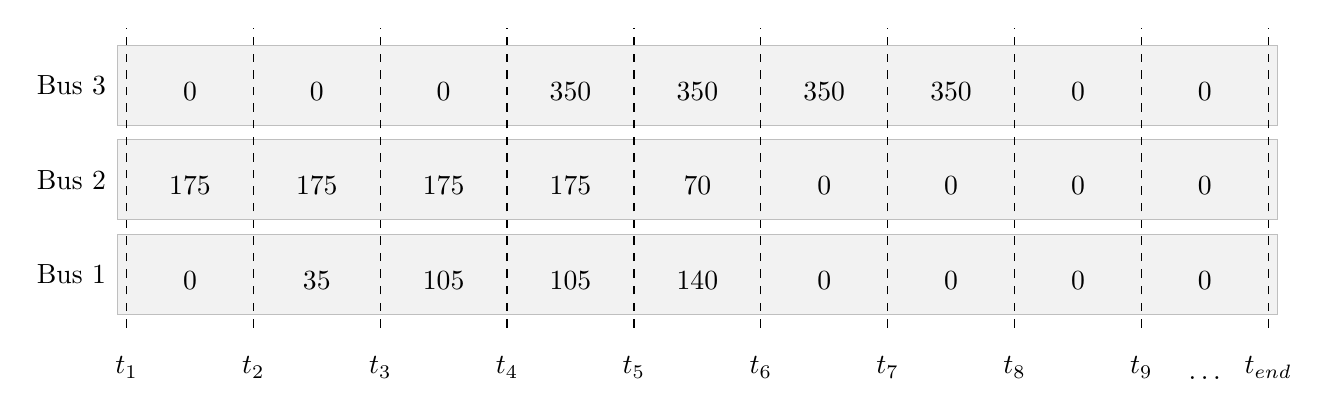
\begin{tikzpicture}
	\node[rectangle, draw=gray!50, fill=gray!10, minimum width=5.8in, minimum height=0.4in](bus1Box) at (7.75,0.8){};
	\node(bus1BoxLabel) at (-0.2, 0.8){Bus 1}; 
	
	\node[rectangle, draw=gray!50, fill=gray!10, minimum width=5.8in, minimum height=0.4in](bus2Box) at (7.75,2){};
	\node(bus1BoxLabel) at (-0.2, 2.0){Bus 2};
	
	\node[rectangle, draw=gray!50, fill=gray!10, minimum width=5.8in, minimum height=0.4in](bus3Box) at (7.75,3.2){};
	\node(bus1BoxLabel) at (-0.2, 3.2){Bus 3};
	
	\foreach \curLab/\preLab[count=\c, evaluate=\c as \pos using {0.5 + (\c - 1)*14.5/9}] in {t_1/t_1, t_2/t_1, t_3/t_2, t_4/t_3, t_5/t_4, t_6/t_7, t_7/t_6, t_8/t_7, t_9/t_8, t_{end}/t_9}
	{
		\node[label=below:$\curLab$](b\c) at (\pos, 0){};
		\node(t) at (\pos, 3.8){};
		\draw[dashed, line width=0.5pt] (b\c.north) -- (t.north); 
		\ifnum\c>1 
			\node(b1Curr) at (\pos, 0.8 - 0.2){};
			\node(b2Curr) at (\pos, 2.0 - 0.2){};
			\node(b3Curr) at (\pos, 3.2 - 0.2){};
			\path(b1Prev.east) -- node(node1\c)[midway, above]{}(b1Curr.west);
			\path(b2Prev.east) -- node(node2\c)[midway, above]{}(b2Curr.west);
			\path(b3Prev.east) -- node(node3\c)[midway, above]{}(b3Curr.west);	
		\fi
			\node(b1Prev) at (\pos, 0.8 - 0.2){};
			\node(b2Prev) at (\pos, 2.0 - 0.2){};
			\node(b3Prev) at (\pos, 3.2 - 0.2){};	
	}
	\path (b9.south) -- node[midway, below=0.1in]{$\hdots$}(b10.south);
	\node at (node12.center){0};
	\node at (node13.center){35};
	\node at (node14.center){105};
	\node at (node15.center){105};
	\node at (node16.center){140};
	\node at (node17.center){0};
	\node at (node18.center){0};
	\node at (node19.center){0};
	\node at (node110.center){0};
	\node at (node22.center){175};
	\node at (node23.center){175};
	\node at (node24.center){175};
	\node at (node25.center){175};
	\node at (node26.center){70};
	\node at (node27.center){0};
	\node at (node28.center){0};
	\node at (node29.center){0};
	\node at (node210.center){0};
	\node at (node32.center){0};
	\node at (node33.center){0};
	\node at (node34.center){0};
	\node at (node35.center){350};
	\node at (node36.center){350};
	\node at (node37.center){350};
	\node at (node38.center){350};
	\node at (node39.center){0};
	\node at (node310.center){0};

\end{tikzpicture}
\caption{An example solution to a 3-bus, 2-charger scenario from $p_4$}
\label{fig:solutionExample}
\end{figure*}

\begin{figure*}
\centering
\scalebox{0.8}{
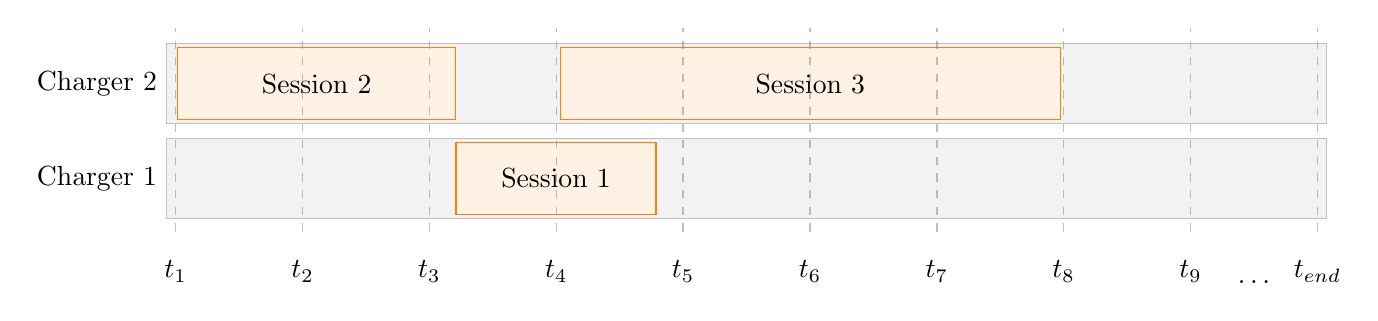
\begin{tikzpicture}
	\node[rectangle, draw=gray!50, fill=gray!10, minimum width=5.8in, minimum height=0.4in](bus1Box) at (7.75,0.8){};
	\node(bus1BoxLabel) at (-0.5, 0.8){Charger 1}; 

	\node[rectangle, draw=gray!50, fill=gray!10, minimum width=5.8in, minimum height=0.4in](bus2Box) at (7.75,2){};
	\node(bus1BoxLabel) at (-0.5, 2.0){Charger 2};
	\node[rectangle, draw=orange!100, fill=orange!10, minimum width=1.3915in, minimum height=0.36in](charge111) at (2.29, 2){Session 2}; 
	\node[rectangle, draw=orange!100, fill=orange!10, minimum width=1in, minimum height=0.36in](charge111) at (5.33, 0.8){Session 1};
	\node[rectangle, draw=orange!100, fill=orange!10, minimum width=2.50in, minimum height=0.36in](charge111) at (8.56, 2){Session 3};


	\foreach \curLab/\preLab[count=\c, evaluate=\c as \pos using {0.5 + (\c - 1)*14.5/9}] in {t_1/t_1, t_2/t_1, t_3/t_2, t_4/t_3, t_5/t_4, t_6/t_7, t_7/t_6, t_8/t_7, t_9/t_8, t_{end}/t_9}
		{
			\node[label=below:$\curLab$](b\c) at (\pos, 0){};
			\node(t) at (\pos, 2.58){};
			\draw[dashed, line width=0.5pt, black!50, opacity=0.5] (b\c.north) -- (t.north); 
		}
		\path (b9.south) -- node[midway, below=0.1in]{$\hdots$}(b10.south); 
\end{tikzpicture}}
\caption{Demonstrates the solution to $p_5$}
\label{fig:secondSolutionExample}
\end{figure*}



\begin{figure*}
\centering
\scalebox{0.8}{
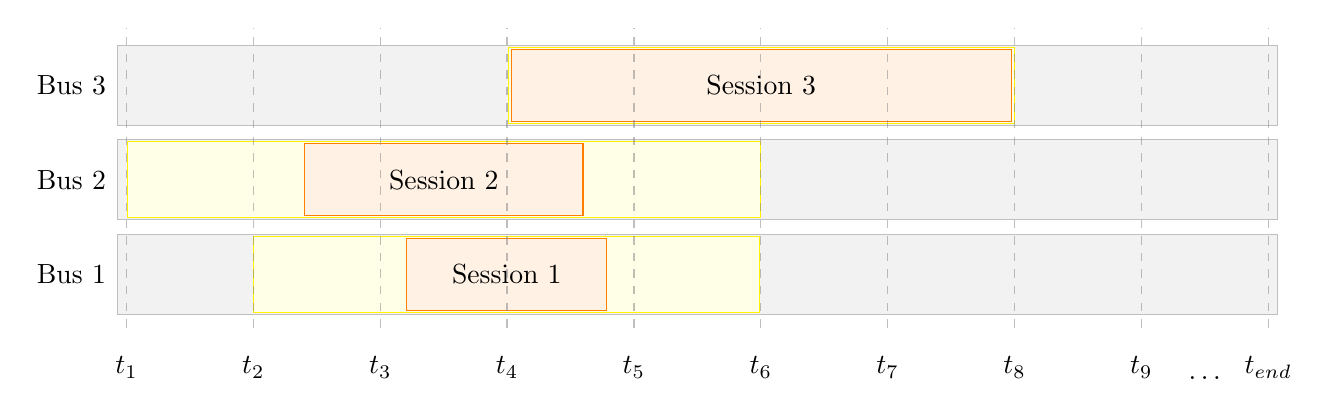
\begin{tikzpicture}
	\node[rectangle, draw=gray!50, fill=gray!10, minimum width=5.8in, minimum height=0.4in](bus1Box) at (7.75,0.8){};
	\node(bus1BoxLabel) at (-0.2, 0.8){Bus 1}; 
	\node[rectangle, draw=yellow!100, fill=yellow!10, minimum width=2.53in, minimum height=0.38in](charge11) at (5.33, 0.8){};
	\node[rectangle, draw=orange!100, fill=orange!10, minimum width=1in, minimum height=0.36in](charge111) at (5.33, 0.8){Session 1};

	\node[rectangle, draw=gray!50, fill=gray!10, minimum width=5.8in, minimum height=0.4in](bus2Box) at (7.75,2){};
	\node(bus1BoxLabel) at (-0.2, 2.0){Bus 2};
	\node[rectangle, draw=yellow!100, fill=yellow!10, minimum width=3.1625in, minimum height=0.38in](charge11) at (4.53, 2){};
	\node[rectangle, draw=orange!100, fill=orange!10, minimum width=1.3915in, minimum height=0.36in](charge111) at (4.53, 2){Session 2};
	
	\node[rectangle, draw=gray!50, fill=gray!10, minimum width=5.8in, minimum height=0.4in](bus3Box) at (7.75,3.2){};
	\node(bus1BoxLabel) at (-0.2, 3.2){Bus 3}; 
	\node[rectangle, draw=yellow!100, fill=yellow!10, minimum width=2.53in, minimum height=0.38in](charge11) at (8.56, 3.2){};
	\node[rectangle, draw=orange!100, fill=orange!10, minimum width=2.50in, minimum height=0.36in](charge111) at (8.56, 3.2){Session 3};


	\foreach \curLab/\preLab[count=\c, evaluate=\c as \pos using {0.5 + (\c - 1)*14.5/9}] in {t_1/t_1, t_2/t_1, t_3/t_2, t_4/t_3, t_5/t_4, t_6/t_7, t_7/t_6, t_8/t_7, t_9/t_8, t_{end}/t_9}
		{
			\node[label=below:$\curLab$](b\c) at (\pos, 0){};
			\node(t) at (\pos, 3.8){};
			\draw[dashed, line width=0.5pt, black!50, opacity=0.5] (b\c.north) -- (t.north); 
		}
		\path (b9.south) -- node[midway, below=0.1in]{$\hdots$}(b10.south); 
\end{tikzpicture}}
\caption{Demonstrates how results from $p_4$ can be reexpressed in terms of continuous variables} 
\label{fig:refactorExample}
\end{figure*}



\begin{figure*}
\centering
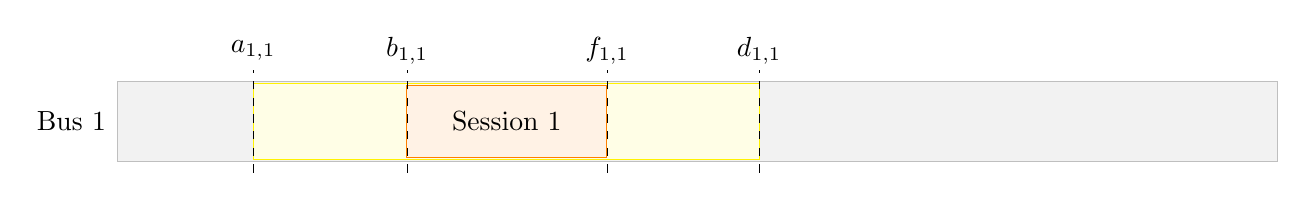
\begin{tikzpicture}
	\node[rectangle, draw=gray!50, fill=gray!10, minimum width=5.8in, minimum height=0.4in](bus1Box) at (7.75,0.8){};
	\node(bus1BoxLabel) at (-0.2, 0.8){Bus 1}; 
	\node[rectangle, draw=yellow!100, fill=yellow!10, minimum width=2.53in, minimum height=0.38in](charge11) at (5.33, 0.8){};
	\node[rectangle, draw=orange!100, fill=orange!10, minimum width=1in, minimum height=0.36in](charge111) at (5.33, 0.8){Session 1}; 
	\draw[dashed] (0.83in,0.15) -- (0.83in,1.45);
	\node at (0.83in,1.7){$a_{1,1}$};
	\draw[dashed] (3.36in, 0.15) -- (3.36in, 1.45);
	\node at (3.36in,1.7){$d_{1,1}$};
	\draw[dashed] (1.6in, 0.15) -- (1.6in, 1.45);
	\node at (1.6in,1.7){$b_{1,1}$};
	\draw[dashed] (2.6in, 0.15) -- (2.6in, 1.45);
	\node at (2.6in,1.7){$f_{1,1}$};
\end{tikzpicture}
\caption{Gives variables of optimization for $p_5$}
\label{fig:secondProgramVars}
\end{figure*} 


\section{Charge Schedules}
The results from the Quadratic Program defined in the previous section give us a general estimate of how much and when buses should charge, however we must still address two primary issues. The first is defining concrete continuous time start and stop times for each charge sessionand the second is limiting the charge sessions to a finite number of chargers. After solving the first program, we take the results and derive {\it preliminary} intervals and average power consumptions for each charge session.  For example, consider a solution to a three bus, two charger scenario given in Fig. \ref{fig:solutionExample}.
Note that there appears to be three buses charging at the same time from $t_5$ to $t_6$ even though there are only two chargers.  We can reformulate this solution in terms of continuous start and stop variables and a variable charge rate so that the {\it duration} of each charge session may be relaxed. The objective is to store the given energy in the corresponding bus within the given charge interval.  Note how few of the charge sessions utilize the chargers to full capacity. This implies that there exists a smaller charge window in which equivalent power can be delivered. This allow us to use the charge durations from the solution from Fig. \ref{fig:solutionExample} as bounds on {\it allowable} charge windows instead of absolute truth. An example of how Fig. \ref{fig:solutionExample} may be reformulated is given in Fig. \ref{fig:refactorExample}. Note how the actual charge sessions don't necessarily need to take up all the time they were initially allocated in the first solution and that these times can fluctuate if the average charge rate is less than the maximum charger capacity. In this example, we assume a maximum charge capacity of 350kW.  Note how the third charge session does have to be exactly where it was scheduled because the average is equal to the maximum charge rate.
If we examin just the schedule for Bus 1, we note that there are four essential variables for the corresponding charge session: $a(i,r)$, $b(i,r)$, $f(i,r)$ and $d(i,r)$ which represent the minimum start time, actual start time, actual end time, and maximum end time respectively. The problem we must now solve is one of arranging these ``rectangles'' such that each one is larger than it's minimum width (or charge time).  We must also account for the number of chargers. It can be helpful to view the problem as a bin packing problem, where each session must fit within the ``swim lane'' of a charger.  For example, taking the charge sessions given in Fig. \ref{fig:refactorExample} and arranging them so that there is no overlap between sessions will yield a valid solution as shown in Fig. \ref{fig:secondSolutionExample}.
\par From Fig. \ref{fig:secondProgramVars}, we know that $a(i,r), b(i,r),f(i,r)$ and $d(i,r)$ must be such that 
\begin{equation*}\begin{aligned}
	a(i,r) \le b(i,r) \\
	b(i,r) \le f(i,r) \\
	f(i,r) \le d(i,r). 	
\end{aligned}\end{equation*}
Where $a(i,r)$ and $d(i,r)$ are known from the previous optimization problem, and $b(i,r)$ and $f(i,r)$ are optimization variables.
\par We desire to solve this second optimization method in a greedy fashion using a heuristic approach. Let $\mathcal{B}$ be the set of all charge sessions which are sorted according to their {\it latest} start time.  Begin by removing the first, or earliest, $n_{\text{charger}}$ sessions and placing them in separate queues for a charger. For the remainder of the charge sessions, we remove the next item from the list, determine which chargers are available to service this request by checking that the previous service can finish before the next will start, and then select the charger which yields the smallest amount of overlap in session availability.
\begin{algorithm}[!ht]
\DontPrintSemicolon
\KwIn{Sorted List of Charge Sessions}
\KwOut{Charge Schedule for Each Charger}
\For{i = 1:$n_{\text{charger}}$}
{
	charger[i].append(inputList.pop())
}
\While{inputList not empty}
{
	item = inputList.pop()\;
	\For{i = 1:$n_{\text{charger}}$}
	{
		bestOverlap = inf\;
		bestCharger = -1\;
		\If{charger $i$ is available}		
		{
			\If{overlap is less than bestOverlap}
			{
				bestOverlap = itemOverlap\;
				bestCharger = i\;
			}
		}
	}
	charger[bestCharger].append(item)\;
}
\caption{Pseudocode that illustrates how charge sessions are assigned}
\label{alg:chargeAssign}
\end{algorithm}

%\input{8_results.tex}
%\input{9_future.tex}
\section*{Acknowledgment}This material is based in part upon work supported by the National Science Foundation through the ASPIRE Engineering Research Center under Grant No. EEC-1941524, the Department of Energy through a prime award with ABB under Grant No. DE-EE0009194, and PacifiCorp under contract number 3590. Any opinions, findings, and conclusions or recommendations expressed in this material are those of the authors and do not necessarily reflect the views of the National Science Foundation, the Department of Energy, or Pacificorp.
%\newpage 
\onecolumn	
\newcommand{\coloredhline}{\arrayrulecolor{gray!20} \hline \\[0.01in]\arrayrulecolor{black}}
\newcommand{\myendline}{\\ \coloredhline}
\label{tab:paperVariables}
\centering
\begin{supertabular}{b{0.06\textwidth} m{0.3\textwidth} m{0.09\textwidth} m{0.06\textwidth} m{0.3\textwidth} m{0.09\textwidth}}
	\toprule%----------------------------------------------------------------------------
	\textbf{Variable} & \textbf{Description} & \textbf{Range} & \textbf{Variable} & \textbf{Description} & \textbf{Range}\\
	\toprule%-----------------------------------------------------------------------------
	\multicolumn{6}{l}{Indices} \myendline
	i & Bus index     & $\mathbb{N}$ & j & Time Index & $\mathbb{N}$\\ \myendline
	k & Charger index & $\mathbb{N}$ & r & Route Index \\[0.15in]
	\hline \\[-5pt]
	\multicolumn{6}{l}{Formulation} \\[-9pt]\myendline
	$n_{\text{bus}}$&\parbox{0.3\textwidth}{The number of buses in the optimization framework.}                                                           & $\mathbb{Z}$            & $n_{\text{time}}$                      &\parbox{0.3\textwidth}{ The number of time indices in a day.                                                                                 }      & $\mathbb{Z}^+$ \\\myendline
	$b_{p(i,j)}$   & \parbox{0.3\textwidth}{The average power consumed by bus $i$ during time period $j$.}                                                                              & $\mathbb{R}$           & $t_j$         &\parbox{0.3\textwidth}{ The time at time index $j$. This paper also refers to the period of time from $t_j$ to $t_{j+1}$ as ``period $t_j$''.}      & $\mathbb{R}$\\\myendline 
	$\bm{b}$       & \parbox{0.3\textwidth}{A vector containing each value for $b_{p(i,j)}$.}                                                                                          & $\mathbb{R}^{n_{\text{bus}}\cdot n_{\text{time}}}$           & $\alpha(i,j)$ &\parbox{0.3\textwidth}{the percentage of time bus $i$ spends in the station from $t_j$ to $t_{j+1}$. }                              & $[0,1]$\\\myendline
	$\mathcal{A}$  & \parbox{0.3\textwidth}{The set of all $i\times j$ elements where bus $i$ can charge at time index $j$}                                  & $i\times j$             & $p_{\text{max}}$ &\parbox{0.3\textwidth}{The maximum power a bus charger can deliver to a bus in kW. This paper assumes a value of 350 for most examples and results.} & $\mathbb{R}^+  $\\\myendline
	$\mathcal{\tilde{A}}$  & \parbox{0.3\textwidth}{The complement of $\mathcal{A}$.}                                                                        & $i\times j$  \\[0.5in]
	\hline \\[-0.07in]
	\multicolumn{6}{l}{Battery} \\[-9pt] \myendline
	$h_{\text{min}}$ & The minimum allowable state of charge                           & $\left ( 0,h_{\text{max}} \right )$                & $h_{\text{max}}$  & The maximum state of charge                                                   & $\mathbb{R}^+$                                     \\ \myendline 
	$\eta_i$         & The beginning state of charge for bus $i$                       & $\left ( h_{\text{min}}, h_{\text{max}} \right )$  & $h(ij)$           & The state of charge for bus $i$ at time $t_j$. & $\left ( h_{\text{min}}, h_{\text{max}} \right )$\\ \myendline
	$\Delta T$       & The change in time from $t_j$ to $t_{j+1}$                      &$\mathbb{R}^+ $  & $\bm{h}$             & A vector containing all state of charge values.                                        & $\mathbb{R}_+^{n_{\text{bus}}\cdot n_{\text{time}}}$                                   \\ \myendline
	$\delta(ij)$     & The battery discharge for bus $i$ during time period $j$.               & $\mathbb{R}_+$                                     & $h(i,\text{end})$& Bus $i$'s final state of charge.                                              & $\left ( h_{\text{min}}, h_{\text{max}} \right )$\\[0.3in]
	\hline \\[-0.07in]
	\multicolumn{6}{l}{Charger Management} \\[-9pt] \myendline 
	$n_{\text{charger}}$             & The time index for the start of bus $i$'s $j^{\text{th}}$ stop                                                    & $\mathbb{Z}_+$                   & $p_c(j)$            & The average power consumed by all buses during time period $j$. & $\mathbb{R}$                    \\ \myendline
	$\bm{p_c}$                       & A vector containing all values of $p_c(j)$.                                                                       & $\mathbb{R}_{+}^{n_{\text{time}}}$                   & $J_{\text{thrash}}$          & A secondary objective function which penalizes multiple plug-in instances per charge session.& $\mathbb{R}_+$                  \\[0.3in] 
	\hline \\[-0.07in]
	\multicolumn{6}{l}{Objective}  \\[-9pt] \myendline
	$\mu_{\text{e-on}}$         & On-Peak Energy Rate                                                            & $\mathbb{R}_+$                                & $\mu_{\text{e-off}}$       & Off-Peak Energy Rate                                                                                     & $\mathbb{R}_+$                 \\ \myendline
	$\mu_{\text{p-on}}$         & On-Peak Demand Power Rate                                                      & $\mathbb{R}_+$                                & $\mu_{\text{p-all}}$       & Facilities Power Rate                                                                                    & $\mathbb{R}_+$                 \\ \myendline
	$\mathcal{S}_{\text{on}}$   & The set of on-peak time indices                                                & \scalebox{0.9}{$\{1,...,n_{\text{time}}\}$}   & $p_{\text{demand}}$        & Maximum average power during on-peak periods                                                             & $\mathbb{R}$                 \\ \myendline
	$p_{\text{facilities}}$     & Maximum average power over all time instances.                                 & $\mathbb{R}_+$                                & $p_t(j)$                   & The total average power co nsumed by both the bus chargers and the uncontrolled loads.                    & $\mathbb{R}_+^{n_{\text{time}}}$  \\ \myendline
	$u(j)$                      & The average power over time $j$ consumed by the uncontrolled loads             & $\mathbb{R}_+^{n_{\text{time}}}$            & $\bm{p}_t$                 & a vector containing $p_t(i)$ for all $i$.                                                                  & $\mathbb{R}_+^{n_{\text{time}}}$ \\ \myendline 
	$e_{\text{on}}$             & The total amount of energy consumed by the bus chargers and uncontrolled loads during off-peak hours.& $\mathbb{R}_+$                              & $e_{\text{off}}$             & The total energy consumed by the bus chargers and uncontrolled loads during on-peak hours.               & $\mathbb{R}_+$ \\ \myendline 
	$J_{\text{cost}}$           & The section of the objective function pertaining to the fiscal expense of charging buses. & $\mathbb{R}$                & $J_{\text{all}}$               & The expression for the complete objective function. & $\mathbb{R}$ \\[0.3in]
	\hline \\[-0.07in]
	\multicolumn{6}{l}{Charge Schedules}  \\[-9pt] \myendline
	$a(i,r)$ & The beginning of the allowable charge interval for bus $i$'s $r^{\text{th}}$ charge session. & $\mathbb{R}_+$ & $b(i,r)$ & The commanded start time for bus $i$'s $r^{\text{th}}$ charge session& $\mathbb{N}$\\ \myendline
	$f(i,r)$ & The commanded end time for bus $i$'s $r^{\text{th}}$ charge session. & $\mathbb{R}_+$ & $d(i,r)$ & The end time of the allowable charge interval for bus $i$'s $r^{\text{th}}$ charge session. & $\mathbb{R}_+$ \\\myendline
	$\sigma(i,r,k)$& A selector variable which is one when bus $i$ charges at charger $k$ for session $r$. & $\{0,1\}$ & $M$ & The number of seconds in a day & $\mathbb{Z}_+$ \\ \myendline
	$l_{(i,r),(i',r')}$ & A selector variable which is one when bus $i$ charges before bus $i'$ during the $r$ and $r'$ sessions respectively. & \scalebox{0.8}{$(i,r) \times (i',r')$} & & & \\ \myendline
	%
\end{supertabular}
\twocolumn

\printbibliography
\end{document}


